\subsection{Simulationserweiterung}
\subsubsection{Steuerung}
Wie im Kapitel Grundlagen \ref{sec_auvSimGrundlage} beschrieben wird in der bestehenden Simulation ein \texttt{lane follower controller}, der ein Linie zwischen einem \textit{old\_waypoint} und einem \textit{new\_waypoint} bildet verwendet.
Die Schnittstelle zur Steuerung bildet also die Kombination aus den beiden Wegpunkten. Die Berechnung der Wegpunkte wird auf Basis des Polynoms aus dem Schätzverfahren generiert.\\
Zunächst wird die Position des AUVs durch die aktuelle Transformationsmatrix transformiert. Es wird der nächste Punkt auf dem Polynom zur transformierten Position des AUVs berechnet. Dieser Punkt dient als Zentrum für einen Kreis zur Bestimmung der Wegpunkte. Mithilfe der Kreisgleichung \todo{ref auf gleichung} werden die zwei Schnittpunkte des Polynoms mit dem Kreis berechnet. Da durch die Transformationsmatrix sichergestellt wird, dass das AUV in Richtung der rotierten $X-Achse$ fährt kann problemlos der Schnittpunkt mit höherem $x$ Wert als \textit{next\_waypoint} und dementsprechend der andere als \textit{old\_waypoint} genommen werden.\\
Der letzte Schritt besteht aus der Transformation der Wegpunkte in das reale VRML-Koordinatensystem mithilfe der inversen Transformationsmatrix.
\todo{Grafik auv kurve kreis old und next waypoint}

\subsubsection{Kamerabilder}
Da die Simulation in der Ursprünglichen Form noch sehr \textit{klinische} Bilder generierte mussten diese Bilder künstlich verschlechtert und die Sichtverhältnisse eingeschränkt werden, um realistische Eingangsbilder zu erzeugen. In Abbildung \ref{simPics} ist von links nach rechts ein ursprüngliches Kamerabild, ein verschlechtertes Bild und ein sehr stark verschlechtertes Bild zu sehen. Die Testläufe der Arbeit wurden mit dem Verschlechterungsgrad des mittleren Bildes durchgeführt. Die Objekterkennung wurde zudem noch mit Bildern, wie dem rechten Bild getestet.

\begin{figure}[H]
\begin{tabular}{ccc}
\subfloat[Ursprüngliches Bild]{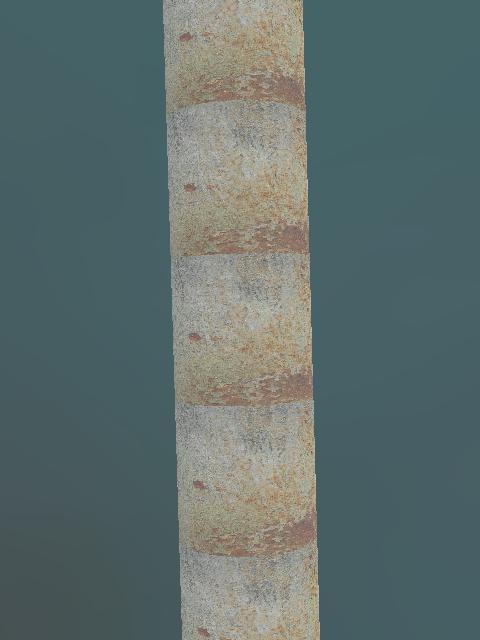
\includegraphics[scale=0.8,width=0.33\textwidth]{/imageProcessing/gradeOptimal.jpg}}&
\subfloat[Künstlich verschlechtertes Bild]{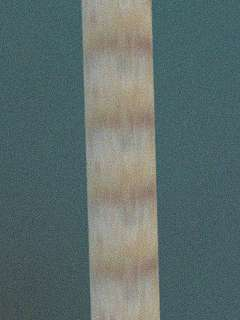
\includegraphics[scale=0.8,width=0.33\textwidth]{/imageProcessing/graeOk.jpg}}&
\subfloat[Sehr stark verschlechtertes Bild]{
\includegraphics[scale=0.8,width=0.33\textwidth]{/imageProcessing/gradeschlecht.jpg}}
\end{tabular}
\caption{Simulationsbilder}
\label{simPics}
\end{figure}